\documentclass[notes]{beamer}

% Preamble
\usetheme{Copenhagen}
\usecolortheme{seagull}
\usefonttheme[onlysmall]{structurebold}
\setbeamerfont{title}{shape=\itshape,family=\rmfamily}
\setbeamertemplate{footline}[frame number]
\usepackage[absolute,overlay]{textpos}
\useinnertheme{circles}
\usepackage{tikz,overpic}
\usetikzlibrary{shapes.geometric, arrows}
\usepackage{courier}
\usepackage{verbatim}
\usetikzlibrary{fit,shapes.misc,arrows, shapes}
\usepackage{varwidth}
\usepackage[latin1]{inputenc}
\usepackage[T1]{fontenc}
\usepackage{libertine}
\usepackage{graphicx}
\PassOptionsToPackage{svgnames}{xcolor}
\usepackage{framed}
\usepackage{animate}
\usepackage{alltt}
\usepackage[lined,boxed,commentsnumbered]{algorithm2e}
\usepackage[space]{grffile}
\usepackage{caption}
\usepackage{listings}
\lstset{
    basicstyle=\small\ttfamily,
    columns=flexible,
    breaklines=true
}
\captionsetup[figure]{labelformat=empty}

\usepackage{tikz}
\tikzstyle{blocktext} = [rectangle, draw, fill=gray!20, 
text width=\textwidth, text centered, 
rounded corners, minimum height=4em]

% put the text at the right corner
\newcommand\FrameText[1]{%
\begin{textblock*}{\paperwidth}(0pt,\textheight)
    \raggedright #1\hspace{.5em}
\end{textblock*}}

% divide slide into 4
\newcommand\FourQuad[4]{%
    \begin{minipage}[b][.35\textheight][t]{.47\textwidth}#1\end{minipage}\hfill%
    \begin{minipage}[b][.35\textheight][t]{.47\textwidth}#2\end{minipage}\\[0.5em]
    \begin{minipage}[b][.35\textheight][t]{.47\textwidth}#3\end{minipage}\hfill
    \begin{minipage}[b][.35\textheight][t]{.47\textwidth}#4\end{minipage}%
}


%quote
\newcommand*\openquote{\makebox(7,3){\scalebox{5.}{``}}}

%for the close quote
%\newcommand*\closequote{\makebox(25,-22){\scalebox{5}{''}}}
\colorlet{shadecolor}{white}
\makeatletter
\newif\if@right
\def\shadequote{\@righttrue\shadequote@i}
\def\shadequote@i{\begin{snugshade}\begin{quote}\openquote}
\def\endshadequote{%
    \if@right\hfill\fi\end{quote}\end{snugshade}}
    %\if@right\hfill\fi\closequote\end{quote}\end{snugshade}}
\@namedef{shadequote*}{\@rightfalse\shadequote@i}
\@namedef{endshadequote*}{\endshadequote}
\makeatother


%change fontsize
\newcommand\Fontvi{\fontsize{6}{7.2}\selectfont}

% title page
\title{\normalsize Chromatin Conformation Prediction from ChIPseq Signal}
       

\author[Lim]
{Ricky Lim\inst{1}} 
\institute[] 
{
    \inst{1}
    Touati Benoukraf-Lab at CSI-NUS
}
\date[22 May 2015]
{CSI-Meeting \\\tiny{mailto:rlim.email@gmail.com}}


\subject{CSI Meeting}

% start presenting...
\begin{document}

\begin{frame}
\titlepage
\end{frame}

\begin{frame}[plain]
    \frametitle{Contents}
    \tableofcontents
\end{frame}


\section{Introduction}
\subsection{Goal}
\begin{frame}
    \frametitle{Chromatin Conformation Prediction}

    \begin{itemize}[<+->]
        \item \textbf{Main Question}: 
            Can we use transcription factor (TF)-ChIPseq to predict protein complexes (direct and indirect bindings) on chromatin?
        \item \textbf{Strategy}: Model ChIPseq signal using Mixture Models to cluster the direct and indirect bindings. 
    \end{itemize}

\end{frame}

\subsubsection{What is ChIPseq?}
\begin{frame}
    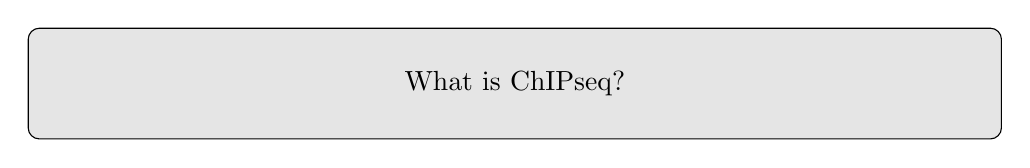
\begin{tikzpicture}[node distance=2cm, auto]
        \node [blocktext] () {What is ChIPseq?};
    \end{tikzpicture}
\end{frame}


{ % ChIP
    \setbeamertemplate{navigation symbols}{}
    \begin{frame}[plain]
        \begin{tikzpicture}[remember picture,overlay]
            \node[at=(current page.center)] {
                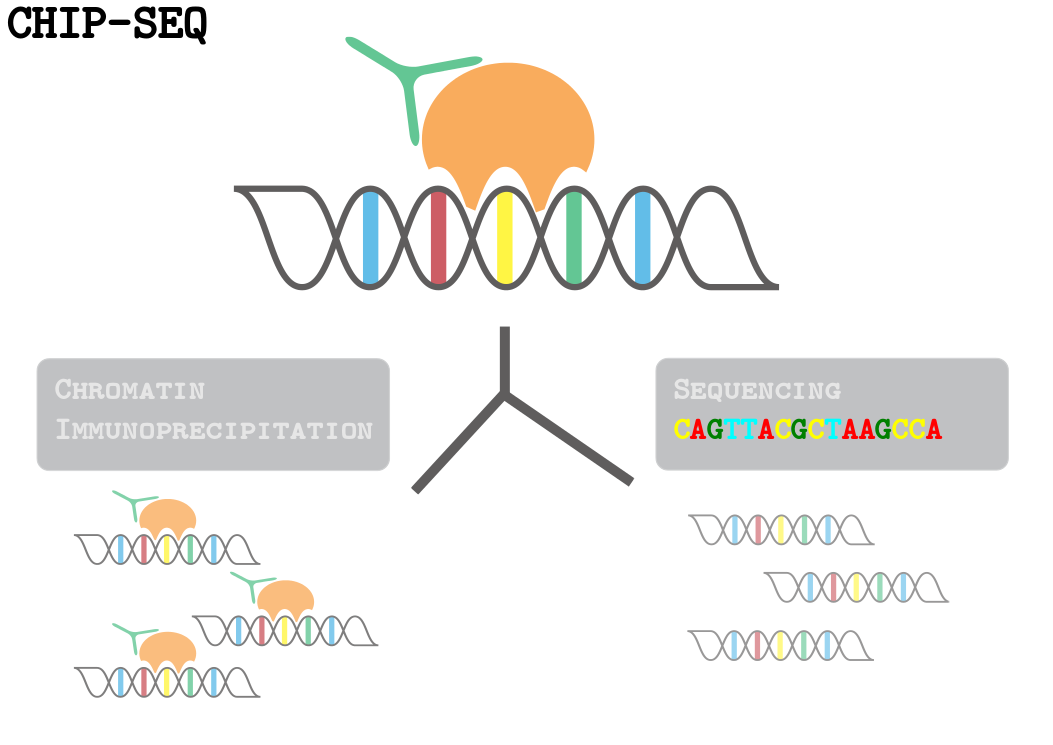
\includegraphics[width=\paperwidth]{../Images/ChIP.png}
            };
        \end{tikzpicture}
     \end{frame}
}

{ % Chromatin Config
    \setbeamertemplate{navigation symbols}{}
    \begin{frame}[plain]
        \begin{tikzpicture}[remember picture,overlay]
            \node[at=(current page.center)] {
                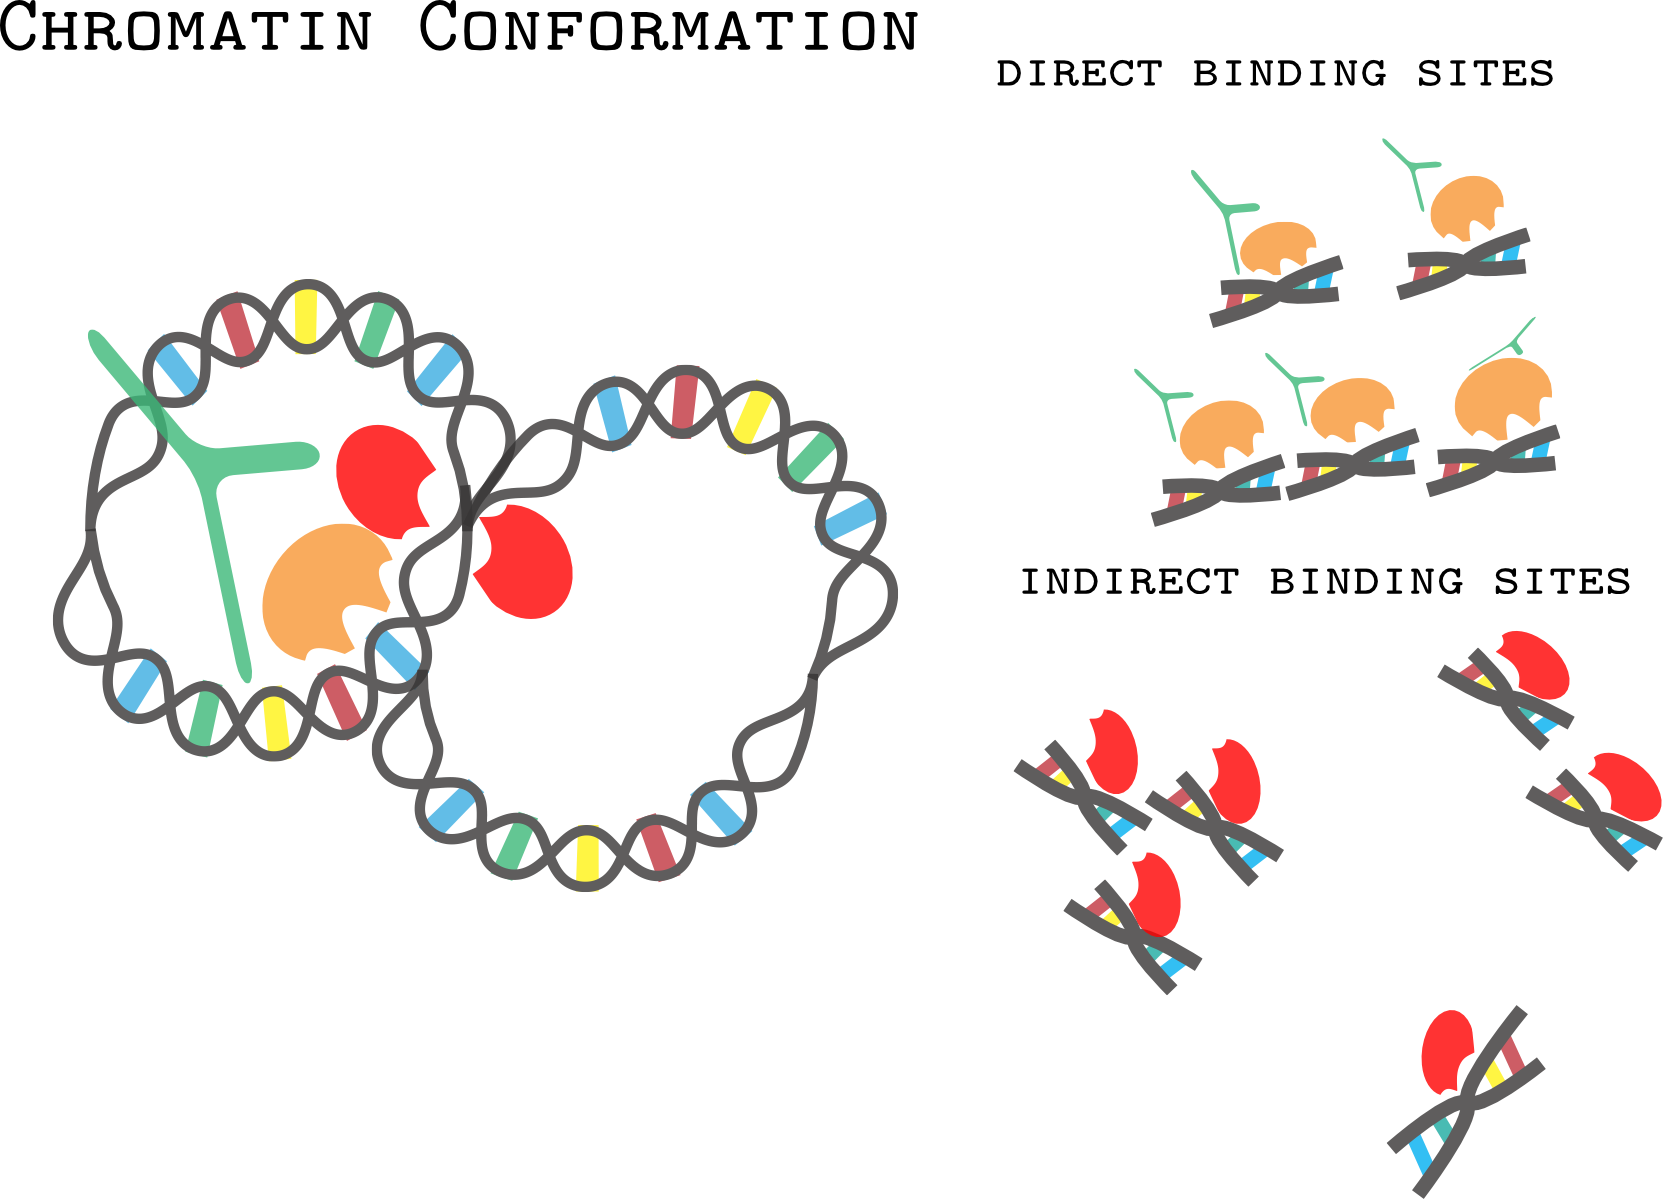
\includegraphics[width=\paperwidth]{../Images/ChromatinConfig.png}
            };
        \end{tikzpicture}

     \end{frame}
}

{ % Chromatin Config
    \setbeamertemplate{navigation symbols}{}
    \begin{frame}[plain]
        \begin{tikzpicture}[remember picture,overlay]
            \node[at=(current page.center)] {
                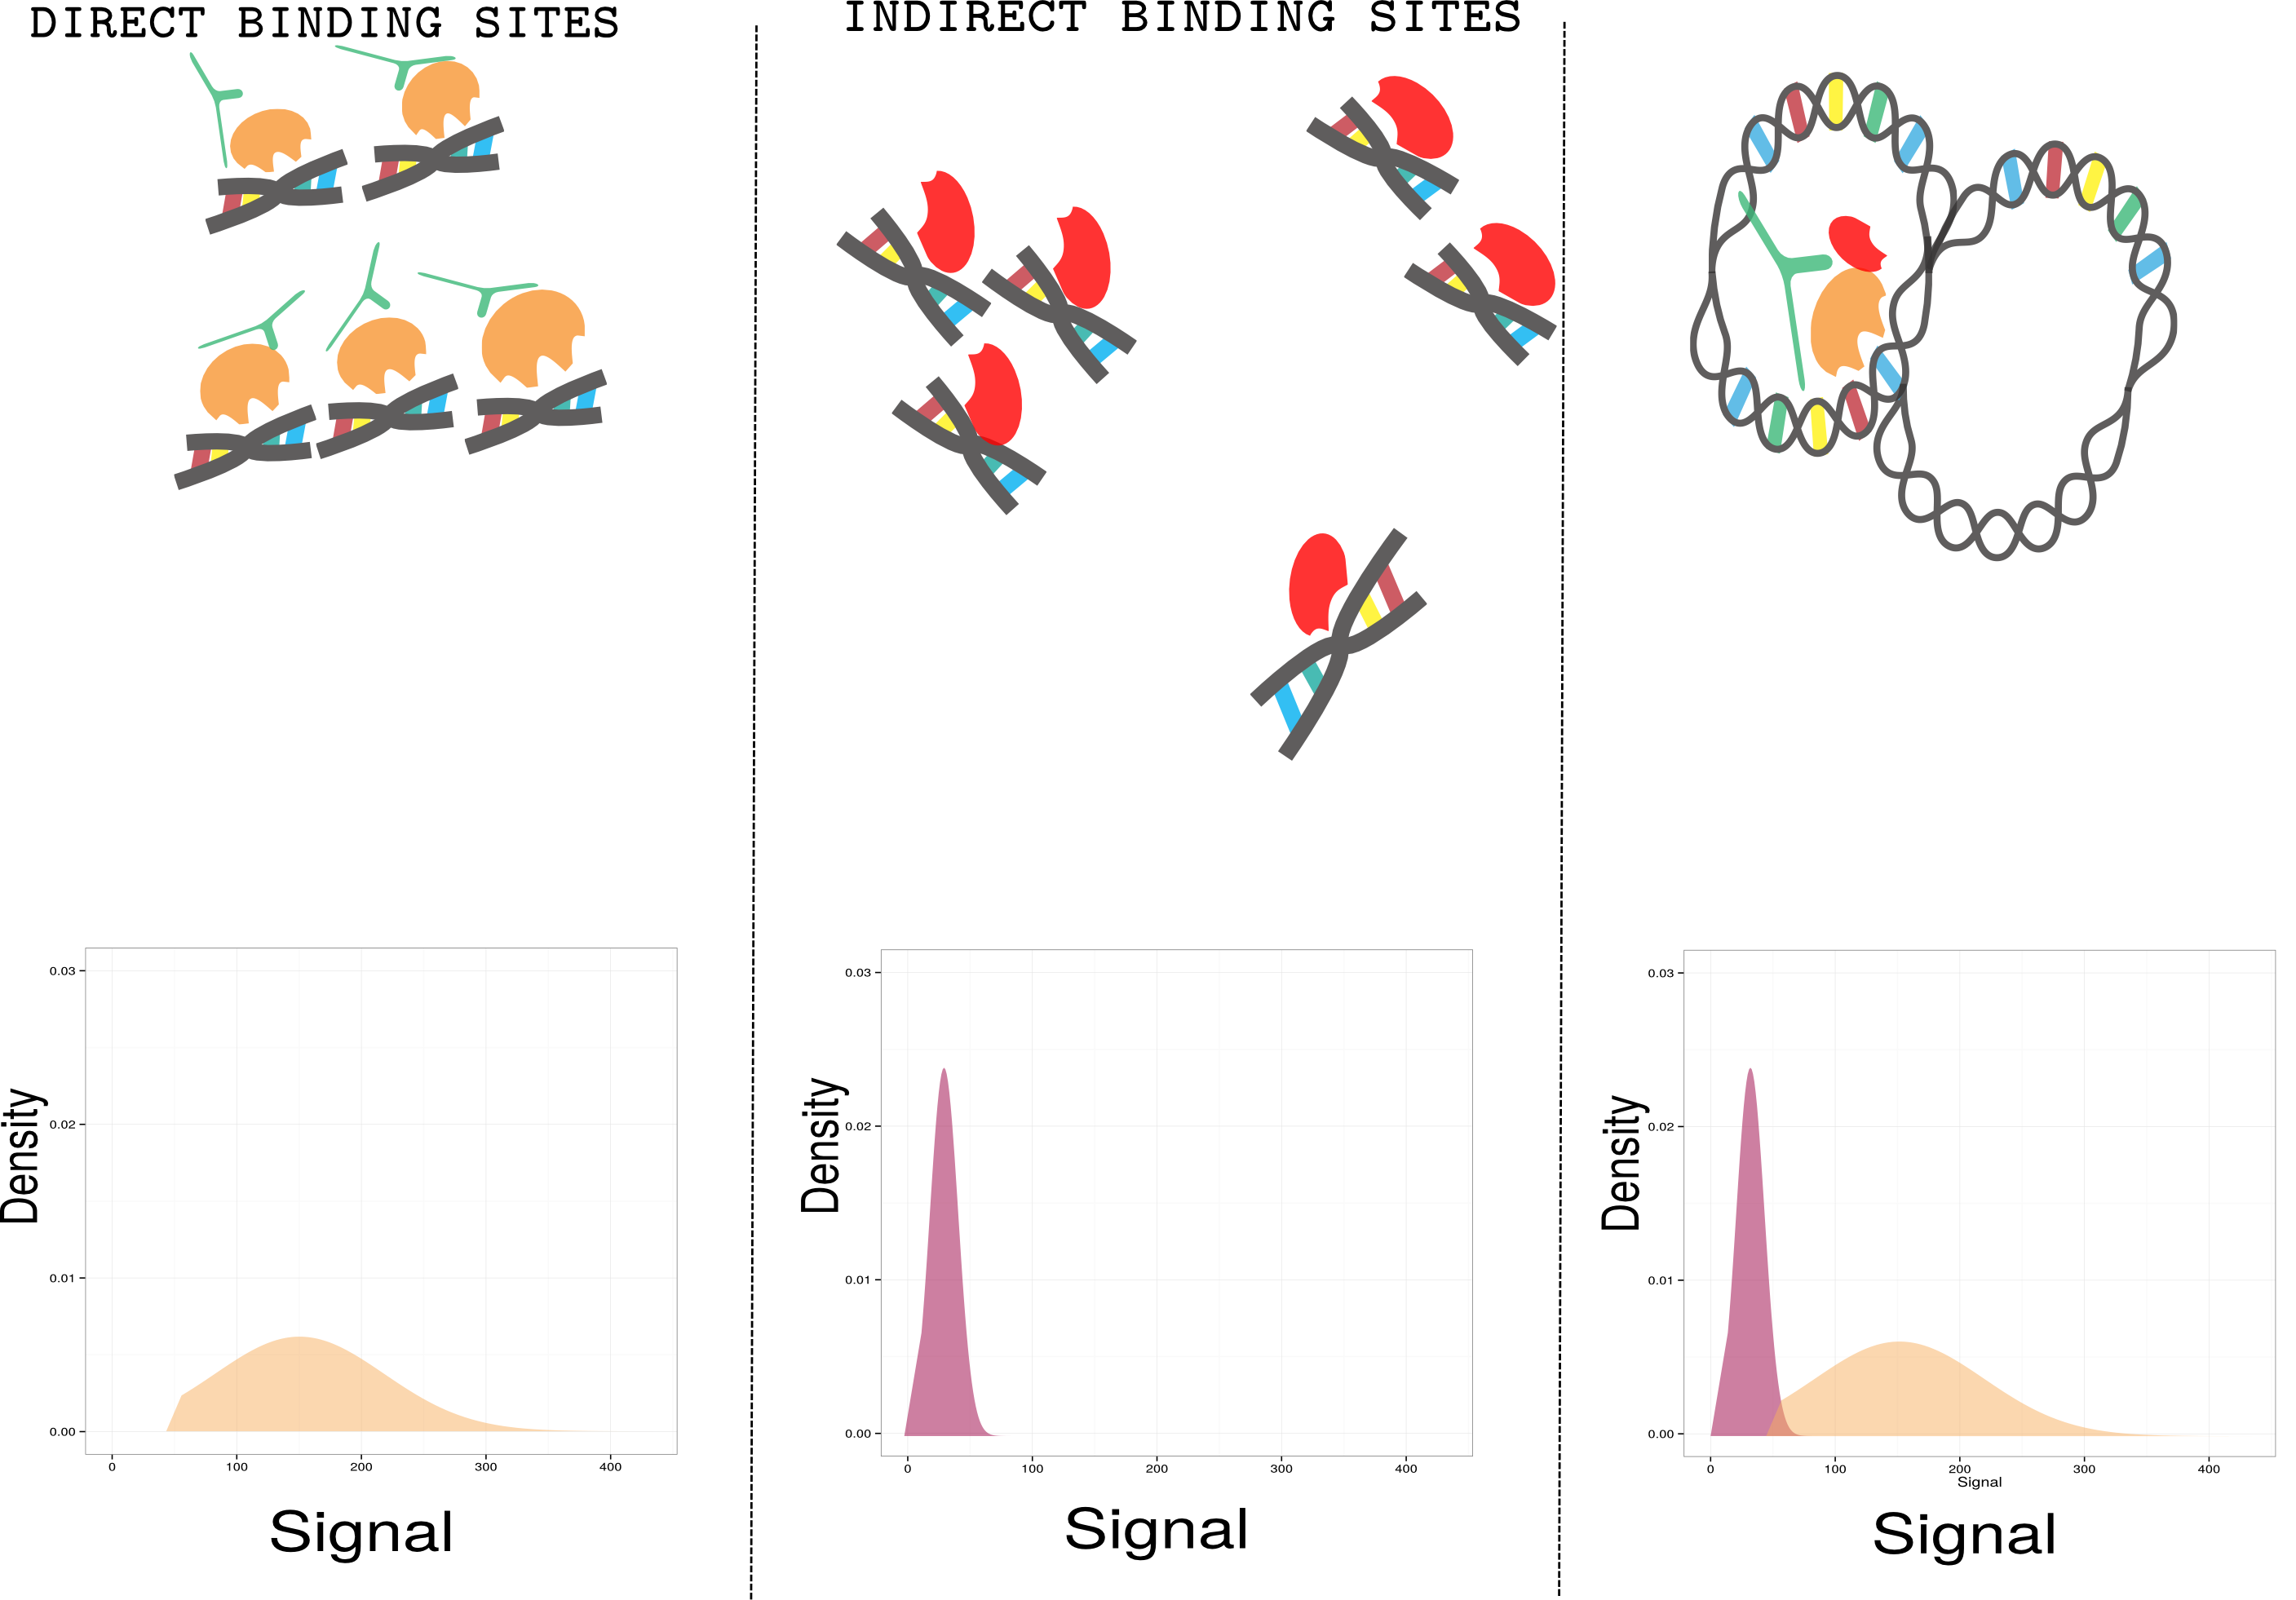
\includegraphics[width=\paperwidth]{../Images/HypotheticalConformation.png}
            };
        \end{tikzpicture}
     \end{frame}
}


\subsubsection{What is Mixture Model?}
\begin{frame}
    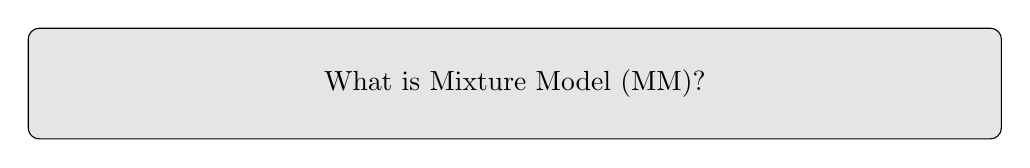
\begin{tikzpicture}[node distance=2cm, auto]
        \node [blocktext] () {What is Mixture Model (MM)?};
    \end{tikzpicture}

\end{frame}

\begin{frame}
    \frametitle{Mixture Model: Revisited}
    Types of clustering methods:
    \begin{itemize}
        \item Hard clustering: non-overlapping clusters
        \item Soft clustering: overlapping clusters
    \end{itemize}

    \vspace{0.1in}
    \pause
    Mixture model is a probabilistic way of soft clustering.
    Each cluster is a generative mixture model with its parameters.


\end{frame}


\begin{frame}[plain]

    \frametitle{Gaussian Mixture Model}
    Key Assumption:\\
    \begin{itemize}
        \item ChIP-seq signals are drawn from a finite set of gaussian distributions.
        \item ChIPseq signals are fit with gaussian mixture models, with mixing $\lambda$ parameter.
        \item Each gaussian corresponds to a cluster of signals with $\mu$ and $\sigma$ parameters.
    \end{itemize}
    \vspace{0.1in}

\end{frame}
                                 

\end{frame}

\section{Our Strategy: Preliminary results}

\subsection{Pipeline}                  
\begin{frame}[plain]
    \begin{center}

    % Define block styles
    \tikzstyle{decision} = [diamond, draw, fill=gray!20, 
        text width=4.5em, text badly centered, node distance=3cm, inner sep=0pt]
    \tikzstyle{block} = [rectangle, draw, fill=gray!80!black,opacity=0.5, 
        text width=5em, text centered, rounded corners, minimum height=4em]
    \tikzstyle{line} = [draw, -latex']
    \tikzstyle{cloud} = [draw, ellipse,fill=red!20, node distance=2cm,
        text width=5em, text centered, minimum height=2em]
        
    \begin{tikzpicture}[node distance = 2cm, auto]
        % Place nodes
        \node [block] (comp) {Component Calls: \small{Mixture Model}};
        \node [block, left of=comp, node distance=3cm, fill=gray!80] (peak) {Peak Calls: \small{MACS \& jaHMM}};
        \node [block, left of=peak, node distance=3cm, fill=green!80,opacity=0.5] (input) {Input: \small{ChIP (*.bam)}};
        \node [block, below of=identify] (assess) {Model Assessment};
        \node [block, right of=assess, node distance=3cm] (update) {Model Update};
        \node [decision, below of=assess] (decide) {Can we identify direct and indirect bindings?};
        \node [block, left of=decide, node distance=5cm] (annot) {Functional Annotation};

        % Draw edges
        \path [line] (comp) -- (assess);
        \path [line] (assess) -- (decide);
        \path [line] (decide) -| node [near start] {no} (update);
        \path [line] (update) |- (comp);
        \path [line] (decide) -- node {yes}(annot);

        \path [line,dashed] (peak) -- (comp);
        \path [line,dashed] (input) -- (peak);
        %\path [line,dashed] (system) |- (assess);
    \end{tikzpicture}

    \end{center}
\end{frame}

\subsubsection{Input Data}
\begin{frame}[plain,fragile]
    \frametitle{Input: ChIP-seq of Cebp$\epsilon$ from Koeffler-BM}
    \begin{lstlisting}
    ##FastQC    0.10.1
    >>Basic Statistics  pass
    #Measure    Value   
    Encoding    Illumina 1.5    
    Total Sequences 41586141    
    Sequence length 40  
    #Summary
    PASS    Basic Statistics    
    PASS    Per base sequence quality   
    PASS    Per sequence quality scores 
    WARN    Per base sequence content   
    PASS    Per base GC content 
    PASS    Per sequence GC content 
    PASS    Per base N content  
    PASS    Sequence Length Distribution    
    PASS    Sequence Duplication Levels 
    PASS    Overrepresented sequences   
    WARN    Kmer Content    
    \end{lstlisting}
\end{frame}
    

\subsubsection{Peak Calls: MACS2 vs jaHMM}
\begin{frame}
    \frametitle{Peak Calls: MACS2 vs jaHMM}
    \begin{itemize}
        \uncover<2->{\item \textbf{MACS2}: \textit{poisson} model-based analysis of Peak calls \footnotemark[1]} 
        \uncover<3->{\item \textbf{jaHMM}: \textit{negative binomial} model-based analysis of Peak calls \footnotemark[2]}
    \end{itemize}
            \footnotetext[1]{Zhang et al. Model-based Analysis of ChIP-Seq (MACS). Genome Biol (2008) vol. 9 (9) pp. R137}
            \footnotetext[2]{Filion et al. jahmm: A tool for discretizing multiple ChIP seq profiles. arXiv (2014)}
\end{frame}

\begin{frame}[plain]
    \frametitle{jaHMM fits ChIPseq Signals better than MACS2}
    \begin{figure}
        \includegraphics[width=0.5\textwidth, height=0.5\textwidth]{/home/ricky/Rlim/ChromatinConformation/ComponentCalls/CebpE/Output/Koeffler_BM_Cebpa_poissonModel.pdf}
        \includegraphics[width=0.5\textwidth, height=0.5\textwidth]{/home/ricky/Rlim/ChromatinConformation/ComponentCalls/CebpE/Output/Koeffler_BM_Cebpa_negBinomModel.pdf}
    \end{figure}
\end{frame}

\begin{frame}[plain]
    \frametitle{Peaks Called by jahmm}
    \begin{figure}
        \includegraphics[width=1\textwidth, height=0.7\textwidth]{/home/ricky/Rlim/ChromatinConformation/PeakCalls/CebpE/Output/KoefflerLab_BM_ChIPseq_CebpE_300_Rjahmm.pdf}
    \end{figure}
\end{frame}

\begin{frame}[plain]
    \frametitle{Peaks Called by MACS2 vs jahmm}
    \begin{figure}                           
        \begin{center}
            \includegraphics[width=1.5in, height=1.5in]{/home/ricky/Rlim/ChromatinConformation/PeakCalls/CebpE/Output/KoefflerLab_BM_ChIPseq_CebpE_macs_jahmm_venn.pdf}
        \end{center}
        \\
        \includegraphics[width=1.5in, height=1.5in]{/home/ricky/Rlim/ChromatinConformation/PeakCalls/CebpE/Output/KoefflerLab_BM_ChIPseq_CebpE_macs_targets.pdf}
        \includegraphics[width=1.5in, height=1.5in]{/home/ricky/Rlim/ChromatinConformation/PeakCalls/CebpE/Output/KoefflerLab_BM_ChIPseq_CebpE_macs_jahmm_targets.pdf}
        \includegraphics[width=1.5in, height=1.5in]{/home/ricky/Rlim/ChromatinConformation/PeakCalls/CebpE/Output/KoefflerLab_BM_ChIPseq_CebpE_jahmm_targets.pdf}
    \end{figure}
\end{frame}

\subsection{Summary: Peak Calls}
\begin{frame}
    \frametitle{Summary: Peak Calls}
    \begin{itemize}[<+->]
        \item Given our dataset, MACS2 is able to call peaks however, the estimated scores are less fit than JAHMM 
        \item Peaks identified solely by jaHMM have scores higher with respect to their input (higher ratio) than solely by MACS2  
    \end{itemize}
\end{frame}

\subsubsection{Component Calls}
\begin{frame}
    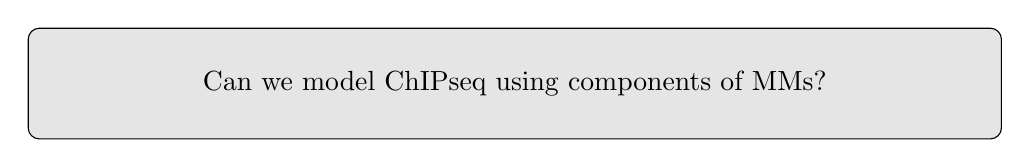
\begin{tikzpicture}[node distance=2cm, auto]
        \node [blocktext] () {Can we model ChIPseq using components of MMs?};
    \end{tikzpicture}

\end{frame}

\begin{frame}
    \frametitle{Input: ChIP-seq of Cebp$\epsilon$ from Koeffler-BM}
    \begin{figure}
        \includegraphics[width=1\textwidth, height=0.6\textwidth]{/home/ricky/Rlim/ChromatinConformation/ComponentCalls/CebpE/ComponentAnalysis/figs/Koeffler_BM_CebpE_CountChipSeqPeaks.pdf}
    \end{figure}
\end{frame}

\begin{frame}                                                                                                                        
    \frametitle{Log Transformation of ChIP-seq Input}
    \begin{figure}
        \includegraphics[width=1\textwidth, height=0.6\textwidth]{/home/ricky/Rlim/ChromatinConformation/ComponentCalls/CebpE/ComponentAnalysis/figs/Koeffler_BM_CebpE_CountChipSeqPeaks_log.pdf}
    \end{figure}
\end{frame}

\begin{frame}                                                                                                                        
    \frametitle{Check the Gaussian Normality}
    \begin{figure}
        \includegraphics[width=0.5\textwidth, height=0.5\textwidth]{/home/ricky/Rlim/ChromatinConformation/ComponentCalls/CebpE/ComponentAnalysis/figs/Koeffler_BM_CebpE_log_qqplot.pdf}
        \includegraphics[width=0.5\textwidth, height=0.5\textwidth]{/home/ricky/Rlim/ChromatinConformation/ComponentCalls/CebpE/ComponentAnalysis/figs/Koeffler_BM_CebpE_qqplot.pdf}
    \end{figure}
\end{frame}


\begin{frame}[plain]
    \frametitle{ComponentCalls: Fit ChIPseq Peaks with GMMs}
    \begin{figure}[!htp]
        \centering
        \subfloat{\includegraphics[width = 1.3in, height = 1 in ]{/home/ricky/Rlim/ChromatinConformation/ComponentCalls/CebpE/ComponentAnalysis/figs/Koeffler_BM_CebpE_GMM_ModelVisualization_log_300_comp2.pdf}}
        \subfloat{\includegraphics[width = 1.3in, height = 1 in ]{/home/ricky/Rlim/ChromatinConformation/ComponentCalls/CebpE/ComponentAnalysis/figs/Koeffler_BM_CebpE_GMM_ModelVisualization_log_300_comp3.pdf}}
        \subfloat{\includegraphics[width = 1.3in, height = 1 in ]{/home/ricky/Rlim/ChromatinConformation/ComponentCalls/CebpE/ComponentAnalysis/figs/Koeffler_BM_CebpE_GMM_ModelVisualization_log_300_comp4.pdf}}
        \\
        \subfloat{\includegraphics[width = 1.3in, height = 1 in ]{/home/ricky/Rlim/ChromatinConformation/ComponentCalls/CebpE/ComponentAnalysis/figs/Koeffler_BM_CebpE_GMM_ModelVisualization_log_300_comp5.pdf}}
        \subfloat{\includegraphics[width = 1.3in, height = 1 in ]{/home/ricky/Rlim/ChromatinConformation/ComponentCalls/CebpE/ComponentAnalysis/figs/Koeffler_BM_CebpE_GMM_ModelVisualization_log_300_comp6.pdf}}
        \subfloat{\includegraphics[width = 1.3in, height = 1 in ]{/home/ricky/Rlim/ChromatinConformation/ComponentCalls/CebpE/ComponentAnalysis/figs/Koeffler_BM_CebpE_GMM_ModelVisualization_log_300_comp7.pdf}}
        \\
        \subfloat{\includegraphics[width = 1.3in, height = 1 in ]{/home/ricky/Rlim/ChromatinConformation/ComponentCalls/CebpE/ComponentAnalysis/figs/Koeffler_BM_CebpE_GMM_ModelVisualization_log_300_comp8.pdf}}
        \subfloat{\includegraphics[width = 1.3in, height = 1 in ]{/home/ricky/Rlim/ChromatinConformation/ComponentCalls/CebpE/ComponentAnalysis/figs/Koeffler_BM_CebpE_GMM_ModelVisualization_log_300_comp9.pdf}}
        \subfloat{\includegraphics[width = 1.3in, height = 1 in ]{/home/ricky/Rlim/ChromatinConformation/ComponentCalls/CebpE/ComponentAnalysis/figs/Koeffler_BM_CebpE_GMM_ModelVisualization_log_300_comp10.pdf}}
    \end{figure}
\end{frame}


\begin{frame}[plain]
    \frametitle{GMM-ModelAssessment: Overfit}
    \begin{figure}[H]
        \centering
        \subfloat{\includegraphics[width = 1.3in, height = 1 in ]{/home/ricky/Rlim/ChromatinConformation/ComponentCalls/CebpE/ComponentAnalysis/figs/Koeffler_BM_CebpE_GMM_ModelVisualization_log_300_comp2_empVsModel.pdf}}
        \subfloat{\includegraphics[width = 1.3in, height = 1 in ]{/home/ricky/Rlim/ChromatinConformation/ComponentCalls/CebpE/ComponentAnalysis/figs/Koeffler_BM_CebpE_GMM_ModelVisualization_log_300_comp3_empVsModel.pdf}}
        \subfloat{\includegraphics[width = 1.3in, height = 1 in ]{/home/ricky/Rlim/ChromatinConformation/ComponentCalls/CebpE/ComponentAnalysis/figs/Koeffler_BM_CebpE_GMM_ModelVisualization_log_300_comp4_empVsModel.pdf}}
        \\
        \subfloat{\includegraphics[width = 1.3in, height = 1 in ]{/home/ricky/Rlim/ChromatinConformation/ComponentCalls/CebpE/ComponentAnalysis/figs/Koeffler_BM_CebpE_GMM_ModelVisualization_log_300_comp5_empVsModel.pdf}}
        \subfloat{\includegraphics[width = 1.3in, height = 1 in ]{/home/ricky/Rlim/ChromatinConformation/ComponentCalls/CebpE/ComponentAnalysis/figs/Koeffler_BM_CebpE_GMM_ModelVisualization_log_300_comp6_empVsModel.pdf}}
        \subfloat{\includegraphics[width = 1.3in, height = 1 in ]{/home/ricky/Rlim/ChromatinConformation/ComponentCalls/CebpE/ComponentAnalysis/figs/Koeffler_BM_CebpE_GMM_ModelVisualization_log_300_comp7_empVsModel.pdf}}
        \\
        \subfloat{\includegraphics[width = 1.3in, height = 1 in ]{/home/ricky/Rlim/ChromatinConformation/ComponentCalls/CebpE/ComponentAnalysis/figs/Koeffler_BM_CebpE_GMM_ModelVisualization_log_300_comp8_empVsModel.pdf}}
        \subfloat{\includegraphics[width = 1.3in, height = 1 in ]{/home/ricky/Rlim/ChromatinConformation/ComponentCalls/CebpE/ComponentAnalysis/figs/Koeffler_BM_CebpE_GMM_ModelVisualization_log_300_comp9_empVsModel.pdf}}
        \subfloat{\includegraphics[width = 1.3in, height = 1 in ]{/home/ricky/Rlim/ChromatinConformation/ComponentCalls/CebpE/ComponentAnalysis/figs/Koeffler_BM_CebpE_GMM_ModelVisualization_log_300_comp10_empVsModel.pdf}}
    \end{figure}
\end{frame}

\begin{frame}
    \frametitle{Model Assessment: BIC-AIC }
        AIC and BIC is based on Occam's razor principle, i.e, the simplest the better.
        \begin{flalign}

        &AIC = $ -2 \times \log L + 2*P  &&

        &BIC = $ -2 \times \log L + \log(n)*P  &&

        &$L$ is likelihood &&

        &$P$ is the number of parameters &&

        \end{flalign}
\end{frame}

\begin{frame}[plain]
    \frametitle{Model Assessment: BIC-AIC}
    \begin{figure}
        \includegraphics[width=0.8\textwidth, height=0.7\textwidth]{/home/ricky/Rlim/ChromatinConformation/ComponentCalls/CebpE/ComponentAnalysis/figs/Koeffler_BM_CebpE_GMM_ModelAssessment_log_300_AICBIC.pdf}
    \end{figure}
\end{frame}

\subsection{Summary: Component Calls}
\begin{frame}
    \frametitle{Summary: Gaussian Mixture Models (GMMs)}
    \begin{itemize}[<+->]
        \item \textbf{Can we model ChIPseq using several components of MMs?}\\
            Yes, our ChIPseq Peaks identified by jaHMM can be fit with GMMs. 

        \item \textbf{How many components are required?}\\
            From AIC-BIC model assessment, 3 components are sufficient to fit ChIPseq signals. 
            \\
            \small{Note: the lower the AIC and BIC values, the better the fitting.}
    \end{enumerate}
\end{frame}

\begin{frame}[plain]
    \begin{center}

    % Define block styles
    \tikzstyle{decision} = [diamond, draw, fill=gray!20, 
        text width=4.5em, text badly centered, node distance=3cm, inner sep=0pt]
    \tikzstyle{block} = [rectangle, draw, fill=gray!80!black,opacity=0.5, 
        text width=5em, text centered, rounded corners, minimum height=4em]
    \tikzstyle{line} = [draw, -latex']
    \tikzstyle{cloud} = [draw, ellipse,fill=red!20, node distance=2cm,
        text width=5em, text centered, minimum height=2em]
        
    \begin{tikzpicture}[node distance = 2cm, auto]
        % Place nodes
        \node [block] (comp) {Component Calls: \small{Mixture Model}};
        \node [block, left of=comp, node distance=3cm, fill=gray!80] (peak) {Peak Calls: \small{MACS \& jaHMM}};
        \node [block, left of=peak, node distance=3cm, fill=green!80,opacity=0.5] (input) {Input: \small{ChIP (*.fastq)}};
        \node [block, below of=identify] (assess) {Model Assessment};
        \node [block, right of=assess, node distance=3cm] (update) {Model Update};
        \node [decision, below of=assess] (decide) {Can we identify direct and indirect bindings?};
        \node [block, left of=decide, node distance=5cm] (annot) {Functional Annotation};

        % Draw edges
        \path [line] (comp) -- (assess);
        \path [line] (assess) -- (decide);
        \path [line] (decide) -| node [near start] {no} (update);
        \path [line] (update) |- (comp);
        \path [line] (decide) -- node {yes}(annot);

        \path [line,dashed] (peak) -- (comp);
        \path [line,dashed] (input) -- (peak);
        %\path [line,dashed] (system) |- (assess);
    \end{tikzpicture}

    \end{center}
\end{frame}


\subsubsection{Motif Calls}
\begin{frame}
    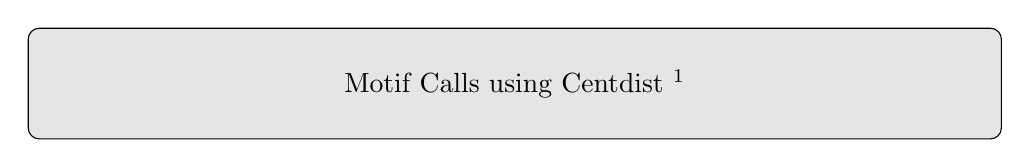
\begin{tikzpicture}[node distance=2cm, auto]
        \node [blocktext] () {Motif Calls using Centdist \footnotemark[1]};
    \end{tikzpicture}
        \footnotetext[1]{Zhang et al. CENTDIST: discovery of co-associated factors by motif distribution. Nucleic Acids (2011)}

\end{frame}


\begin{frame}[plain]
    \frametitle{Group1: low peak score (29559 peaks)}
    \begin{figure}
        \includegraphics[width=1\textwidth, height=0.6\textwidth]{/home/ricky/Rlim/ChromatinConformation/MotifCalls/CebpE/Output/CentDist/Koeffler_BM_CebpE_GMM_ModelAssignment_log_300_group1_compSorted3/top3.png}
    \end{figure}
\end{frame}

\begin{frame}[plain]
    \frametitle{Group2: intermediate peak score (28851 peaks)}
    \begin{figure}
        \includegraphics[width=1\textwidth, height=0.6\textwidth]{/home/ricky/Rlim/ChromatinConformation/MotifCalls/CebpE/Output/CentDist/Koeffler_BM_CebpE_GMM_ModelAssignment_log_300_group2_compSorted3/top3.png}
    \end{figure}
\end{frame}

\begin{frame}[plain]
    \frametitle{Group3: high peak score (5741 peaks)}
    \begin{figure}
        \includegraphics[width=1\textwidth, height=0.6\textwidth]{/home/ricky/Rlim/ChromatinConformation/MotifCalls/CebpE/Output/CentDist/Koeffler_BM_CebpE_GMM_ModelAssignment_log_300_group3_compSorted3/top3.png}
    \end{figure}
\end{frame}

%\begin{frame}
%    \begin{tikzpicture}[node distance=2cm, auto]
%        \node [blocktext] () {Motif Calls using Centrimo};
%    \end{tikzpicture}
%\end{frame}

%\begin{frame}[plain]
%\begin{figure}
%    \subfloat{\includegraphics[width=0.3\textwidth,height=0.3\textwidth]{/home/ricky/Rlim/ChromatinConformation/MotifCalls/CebpE/Output/ChipMeme_Koeffler_BM_CebpE_jahmm300_group1_compSorted3/ChipMeme_Koeffler_BM_CebpE_jahmm300_group1_compSorted3_centrimo.png}}
%    \subfloat{\includegraphics[width=0.3\textwidth,height=0.3\textwidth]{/home/ricky/Rlim/ChromatinConformation/MotifCalls/CebpE/Output/ChipMeme_Koeffler_BM_CebpE_jahmm300_group2_compSorted3/ChipMeme_Koeffler_BM_CebpE_jahmm300_group2_compSorted3_centrimo.png}}
%    \subfloat{\includegraphics[width=0.3\textwidth,height=0.3\textwidth]{/home/ricky/Rlim/ChromatinConformation/MotifCalls/CebpE/Output/ChipMeme_Koeffler_BM_CebpE_jahmm300_group3_compSorted3/ChipMeme_Koeffler_BM_CebpE_jahmm300_group3_compSorted3.png}}
%    \caption{Group 1, 2, and 3 from 3 GMMs left to right}
%\end{figure}
%\end{frame}

\subsection{Summary: Motif Calls}
\begin{frame}
    \frametitle{Summary: Motif Calls}
    \begin{itemize}[<+->]
        \item Cebp motif is found in group 2 and 3 in 3-component GMMS using centdist
        \item Next, can we further segregate these groups into direct and indirect bindings?
    \end{itemize}
\end{frame} 

\subsubsection{Model Update: Biclustering}
{ % Biclustering
    \setbeamertemplate{navigation symbols}{}
    \begin{frame}[plain]
        \begin{tikzpicture}[remember picture,overlay]
            \node[at=(current page.center)] {
                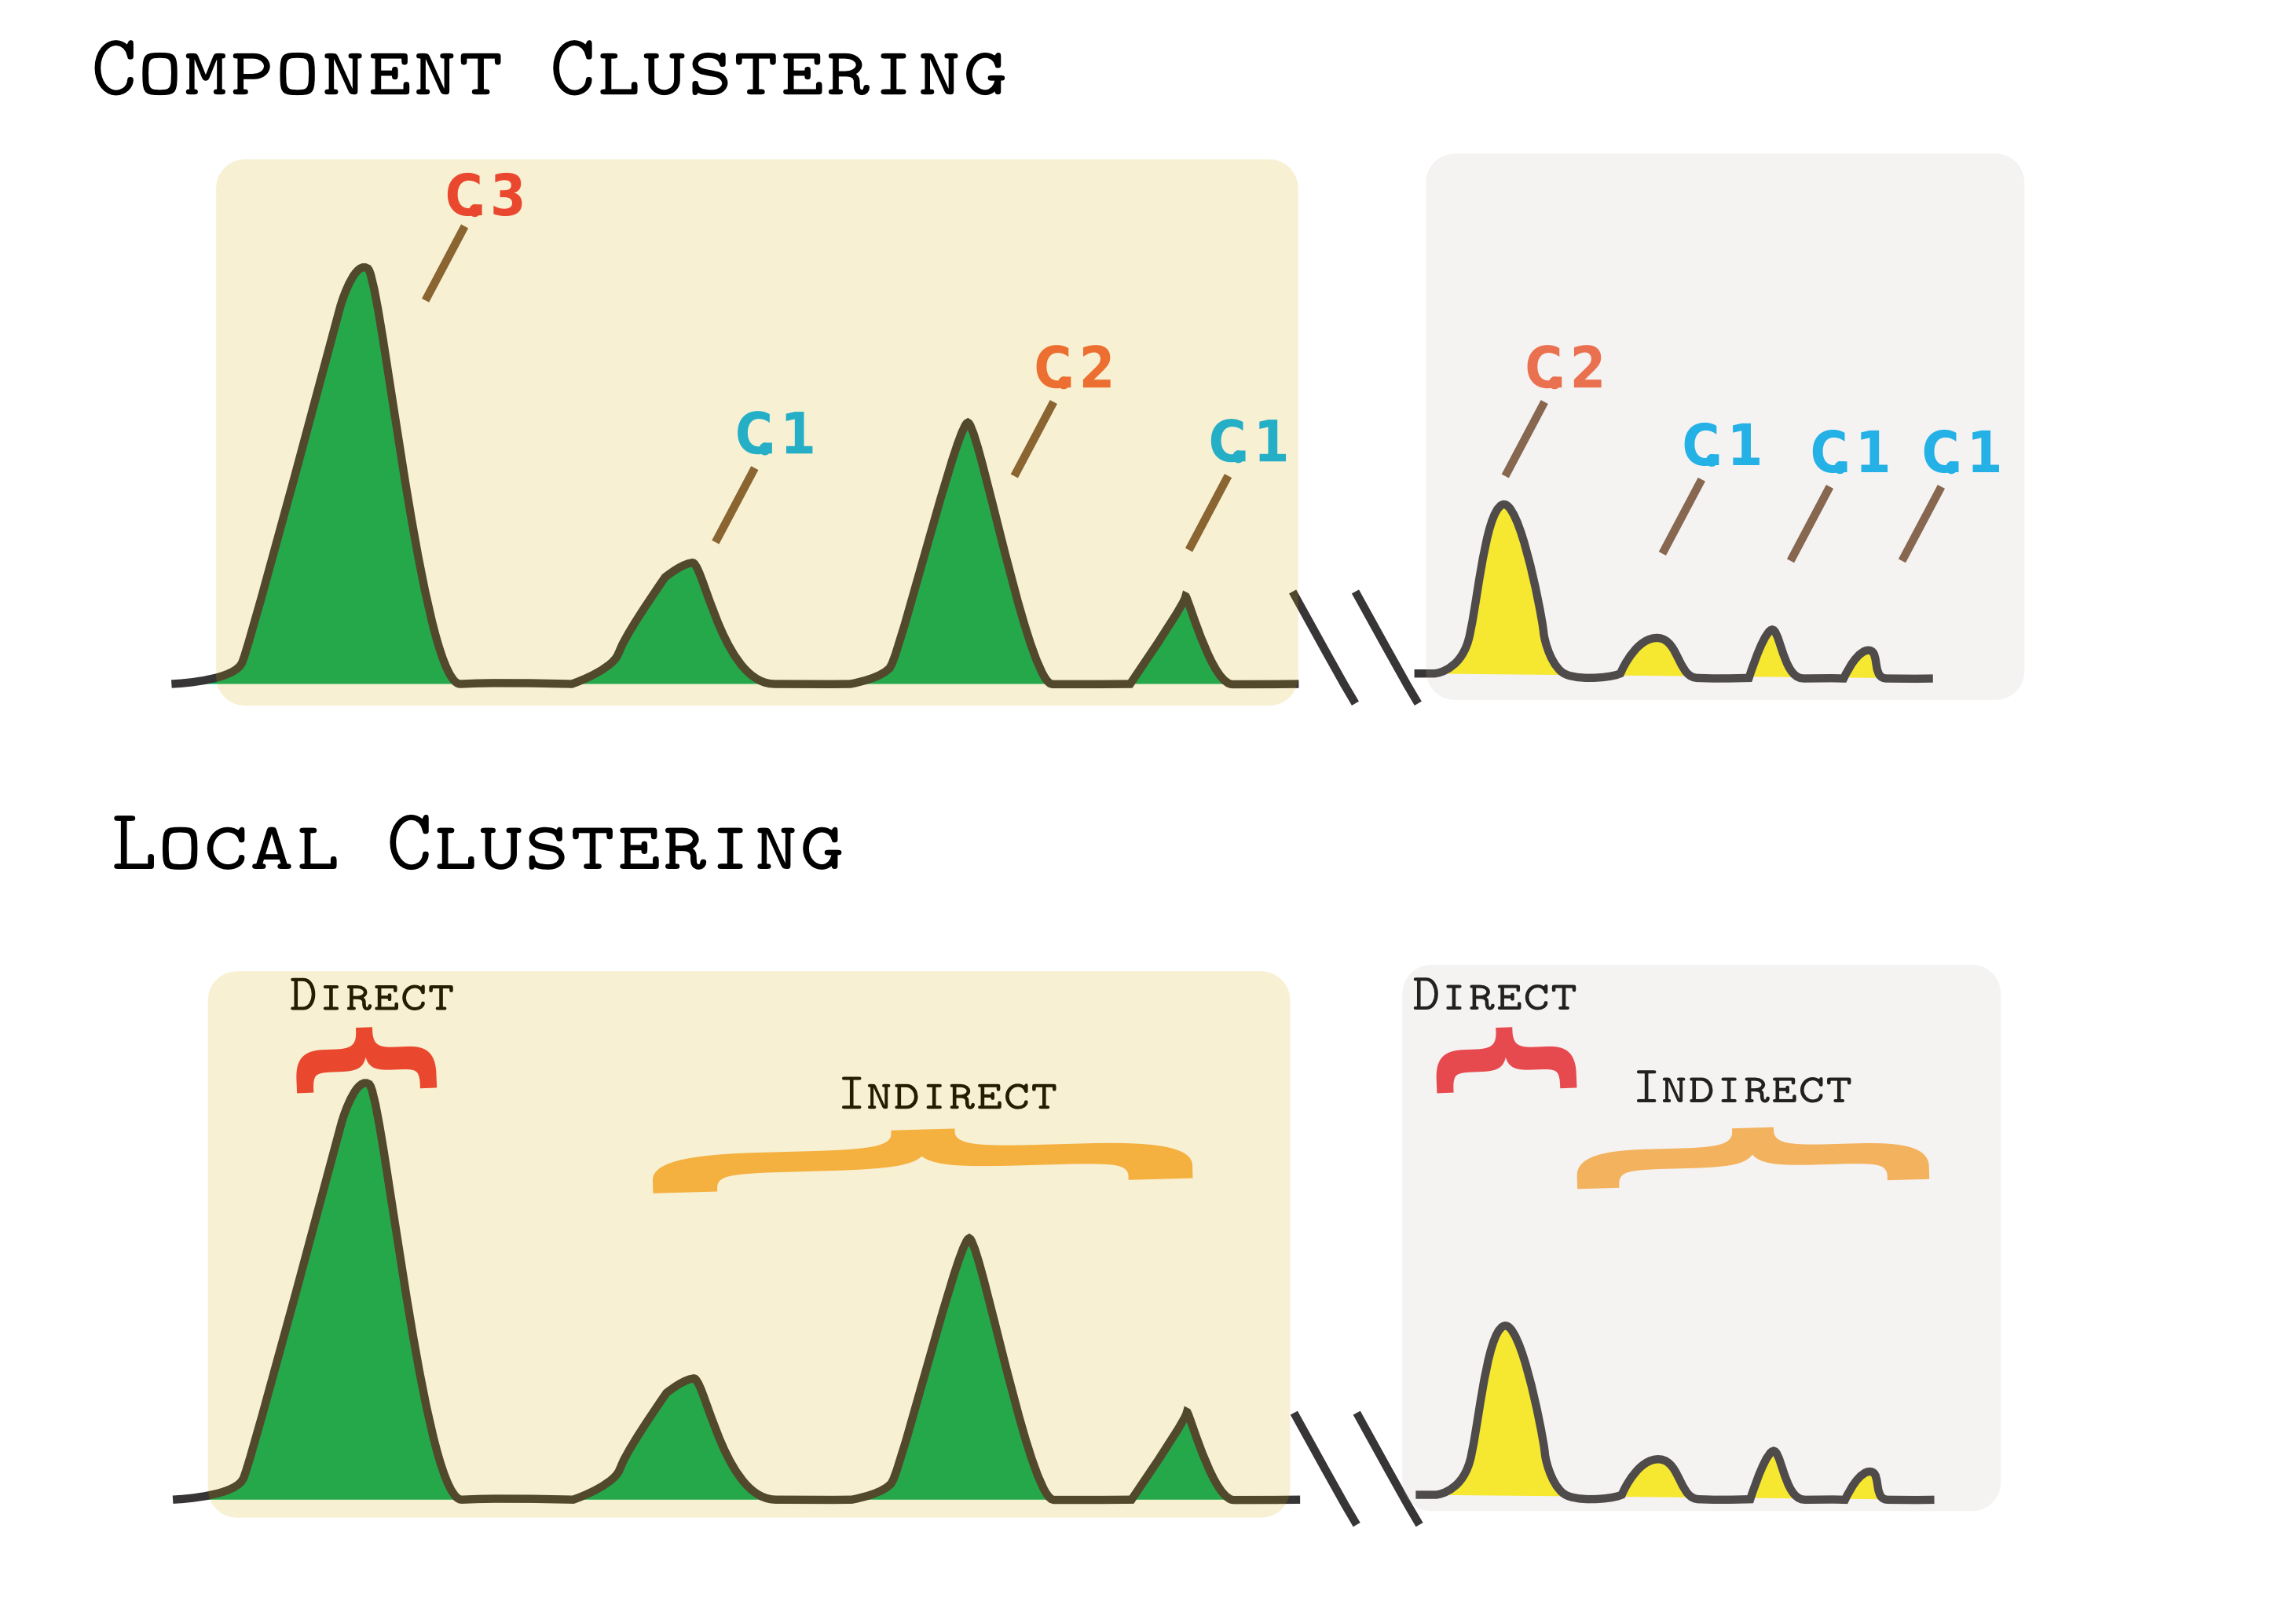
\includegraphics[width=0.8\paperwidth]{../Images/LocalClustering.png}
            };
        \end{tikzpicture}
     \end{frame}
}

\begin{frame}[plain]
    \frametitle{Direct: 24948 peaks}
    \begin{figure}
        \includegraphics[width=1\textwidth, height=0.6\textwidth]{/home/ricky/Rlim/ChromatinConformation/MotifCalls/CebpE/Output/CentDist/Koeffler_BM_CebpE_GMM_BiclusterAssignment_SinglePeakFilteredOut_log_300_compSorted3_dist3kb_direct/top3.png}
    \end{figure}
\end{frame}

\begin{frame}[plain]
    \frametitle{Indirect: 26547 peaks}
    \begin{figure}
        \includegraphics[width=1\textwidth, height=0.6\textwidth]{/home/ricky/Rlim/ChromatinConformation/MotifCalls/CebpE/Output/CentDist/Koeffler_BM_CebpE_GMM_BiclusterAssignment_SinglePeakFilteredOut_log_300_compSorted3_dist3kb_indirect/top3.png}
    \end{figure}
\end{frame}

\section{Summary and Future}
    \begin{frame}
        \begin{itemize}[<+->]
            \item Our current method could separate direct and indirect bindings 
            \item Next, can we further using peak clusters increase functional annotation?
        \end{itemize}
    \end{frame} 

\begin{frame}[plain]
    \begin{figure}
        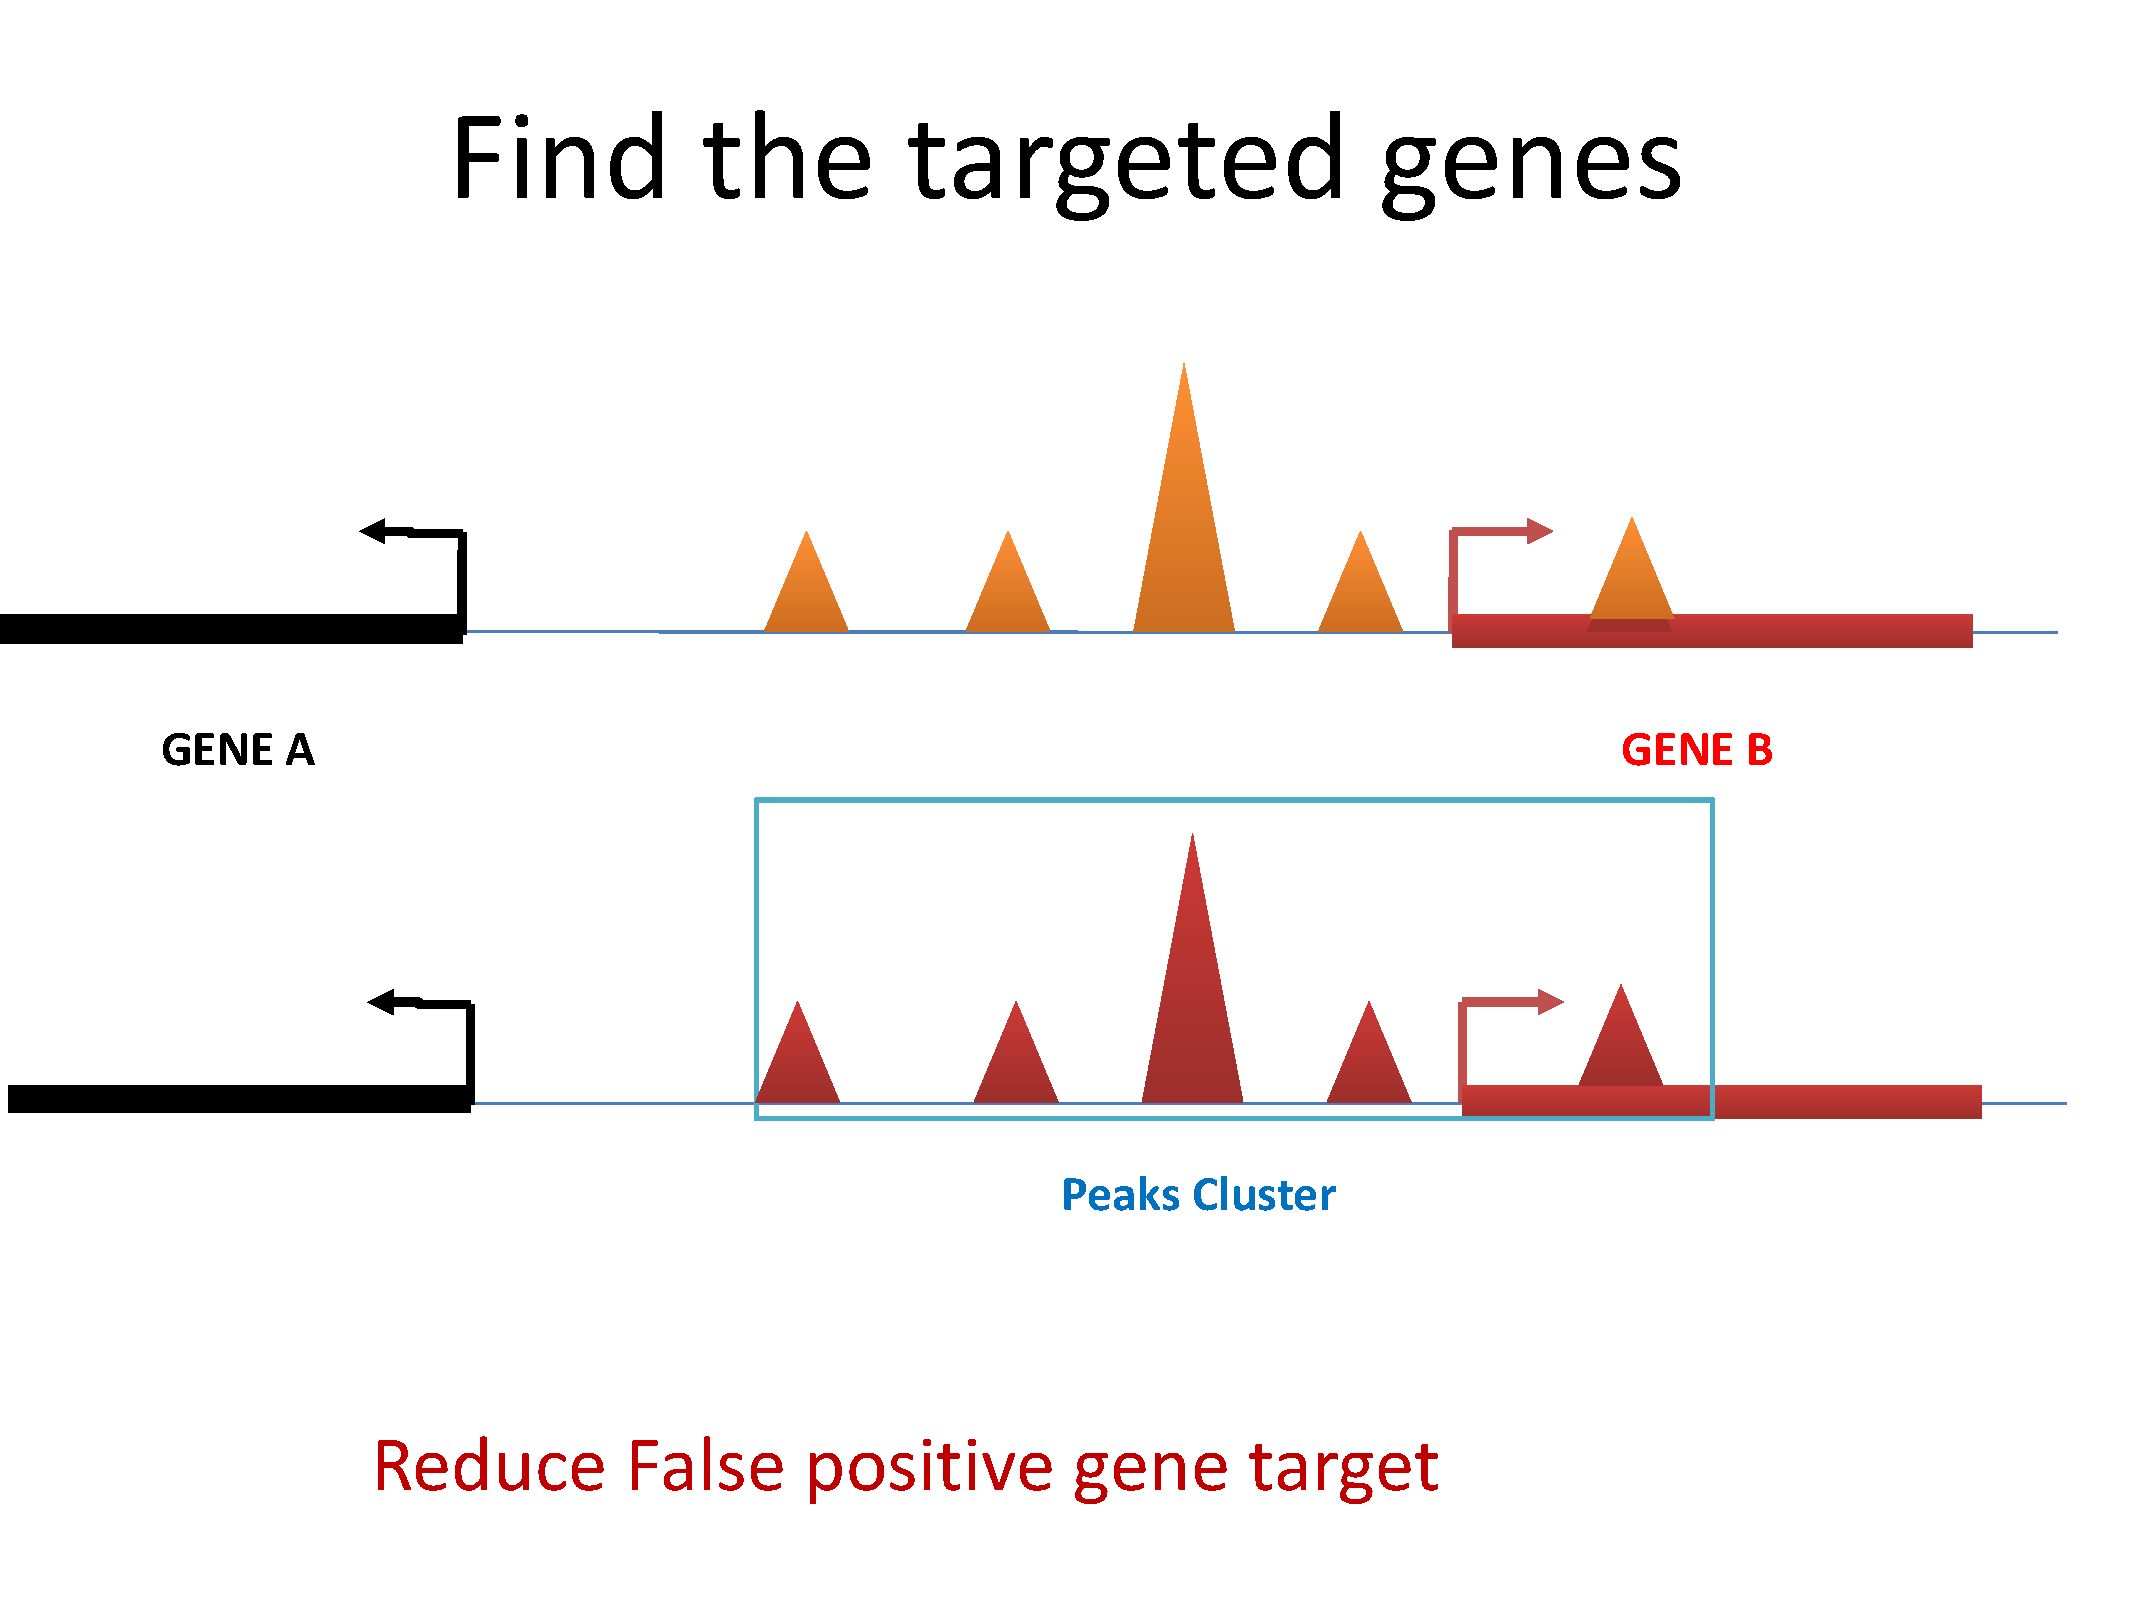
\includegraphics[width=1\textwidth, height=1\textwidth]{/home/ricky/Rlim/Presentations/22.05.15-CSIMeeting/Figures/geneAnnotation_page1.pdf}
    \end{figure}
\end{frame}

\begin{frame}[plain]
    \begin{figure}
        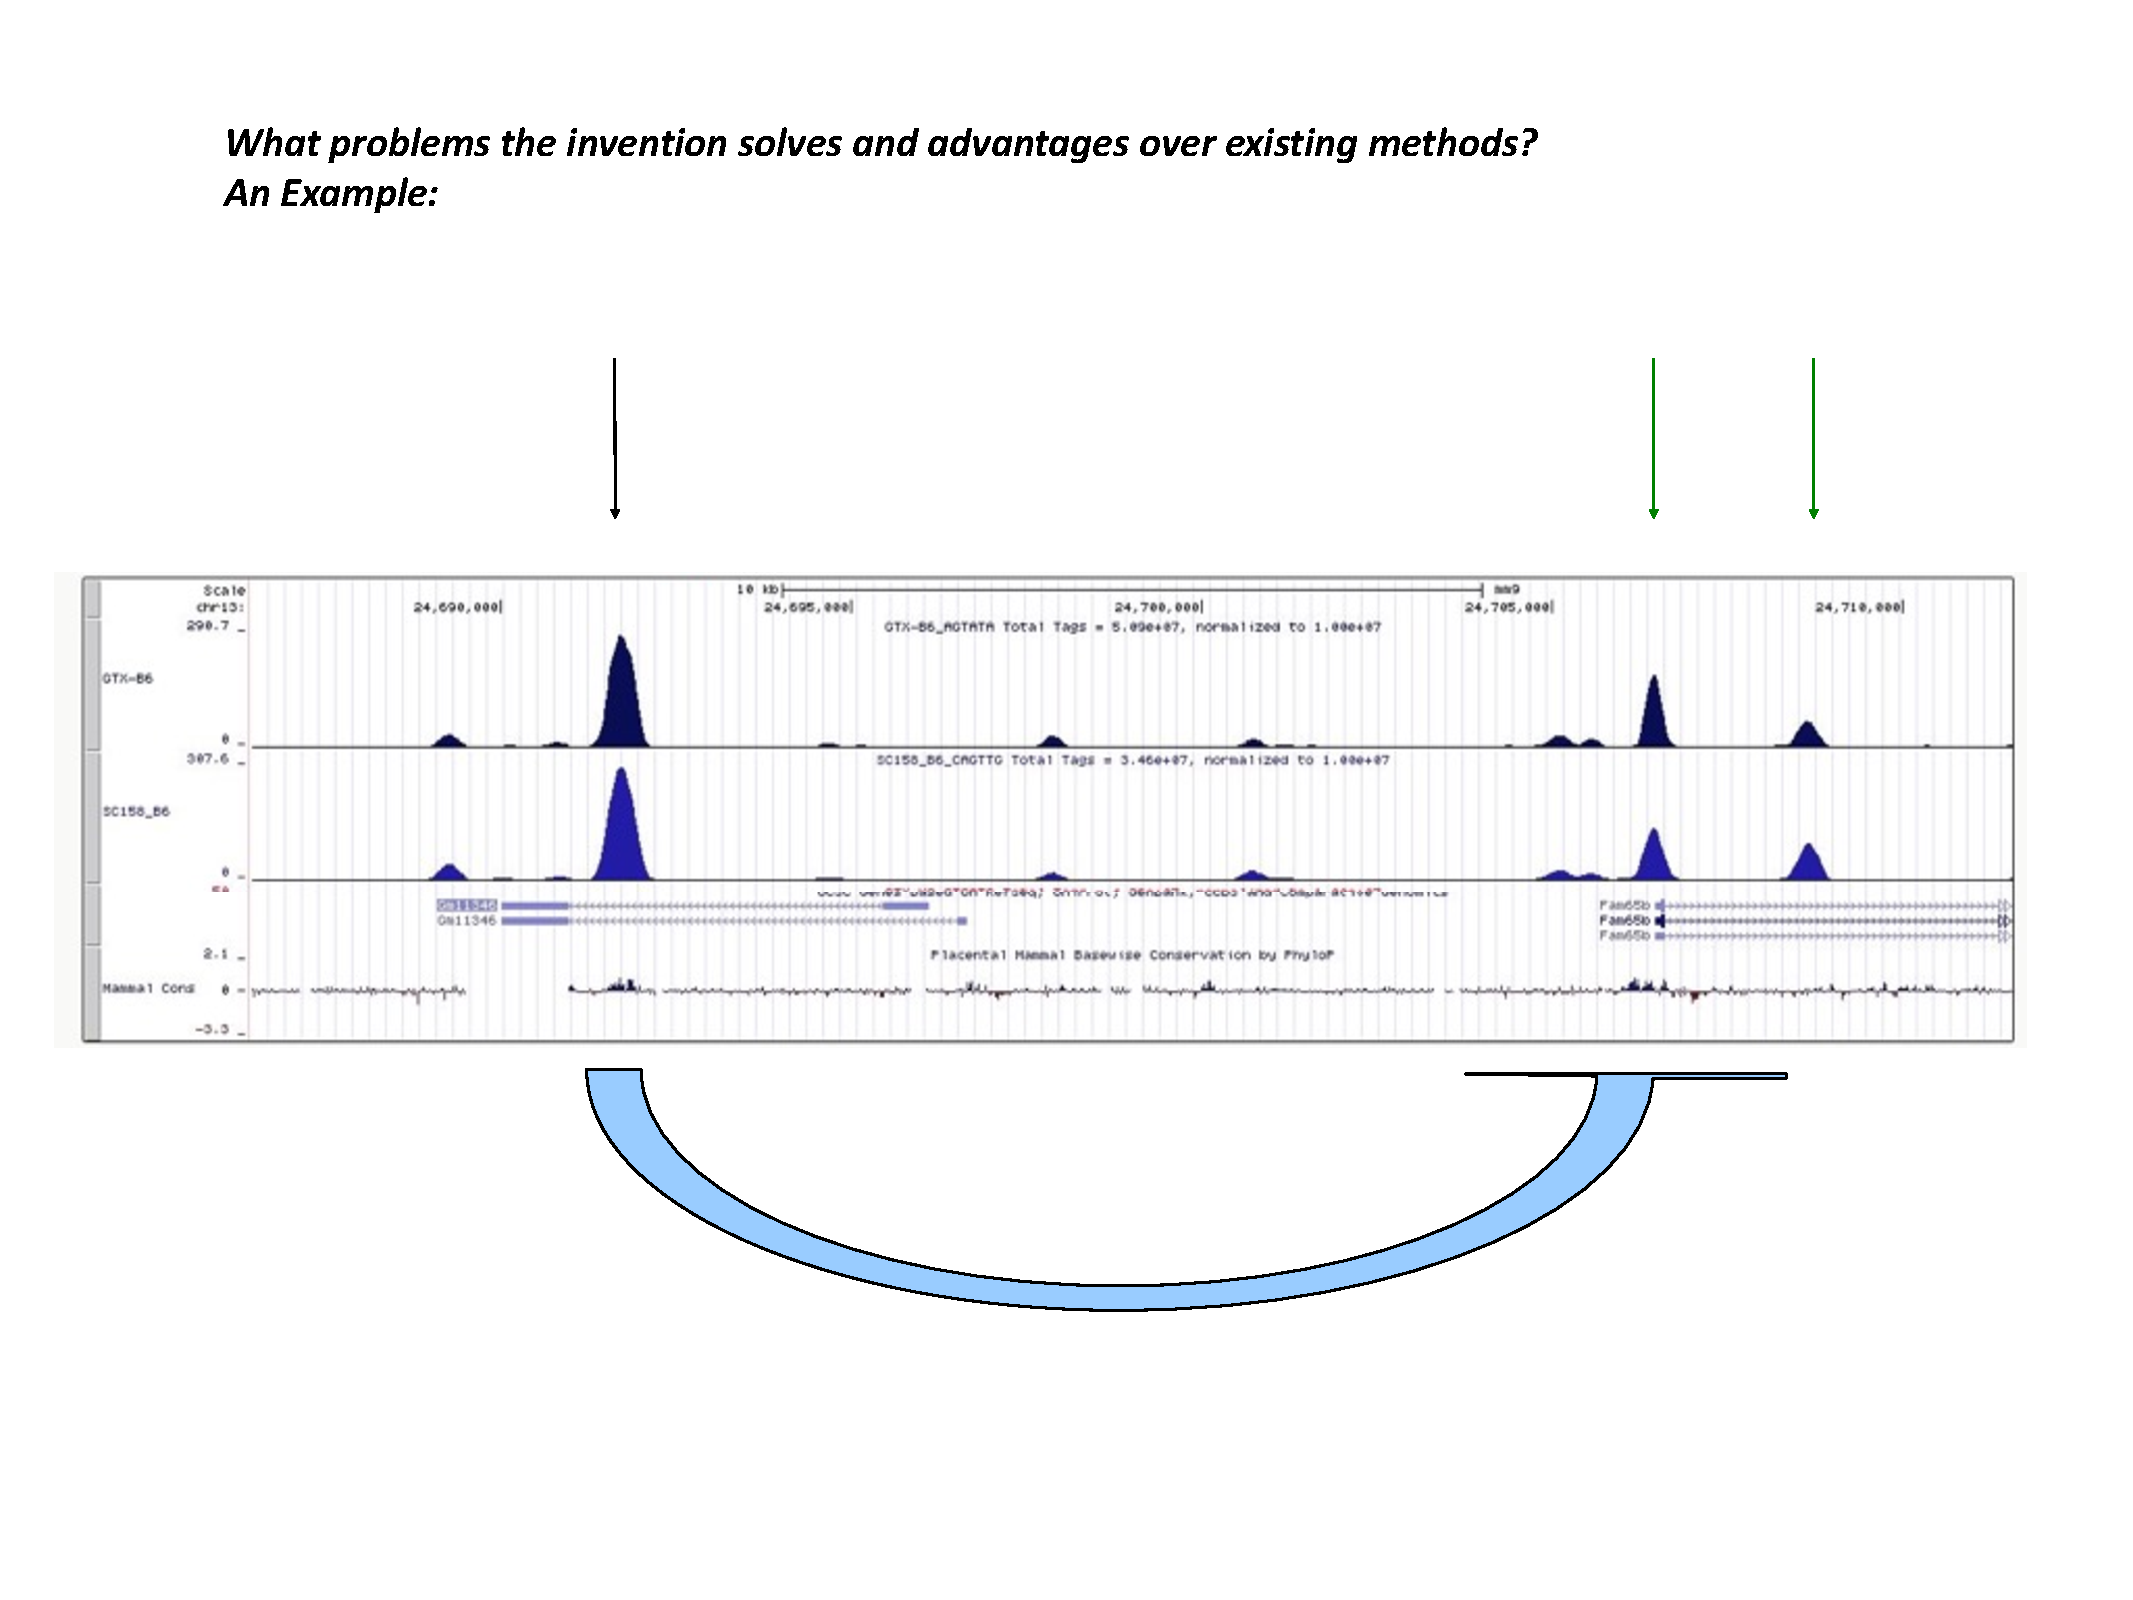
\includegraphics[width=1\textwidth, height=1\textwidth]{/home/ricky/Rlim/Presentations/22.05.15-CSIMeeting/Figures/geneAnnotation_page2.pdf}
    \end{figure}
\end{frame}

\begin{frame}[plain]
    \frametitle{Acknowledgement}
    \begin{itemize}
        \item Touati Benoukraf (CSI-NUS)
        \item Samuel Collombet (Ecole Normale Superieur)
        \item Agus Salim (La Trobe University)
        \item Tong Yin (CEDARS SINAI Hospital)
        \item Phillip Koeffler (CSI-NUS)
    \end{itemize}
\end{frame}


\end{document}
